% Chapter Template

\chapter{State-of-the-art} % Main chapter title

\label{Chapter2} % Change X to a consecutive number; for referencing this chapter elsewhere, use \ref{ChapterX}

\lhead{Chapter 2. \emph{State-of-the-art}} % Change X to a consecutive number; this is for the header on each page - perhaps a shortened title

%----------------------------------------------------------------------------------------
%	SECTION 1
%----------------------------------------------------------------------------------------
\section{Introduction}
This chapter will review research literature in the field of machine learning and credit scoring. We 


%----------------------------------------------------------------------------------------
%	SECTION 2
%----------------------------------------------------------------------------------------
\section{Location/Geospatial Data in Predictive Modelling}
The geography of the data  Provinces  Ireland is divided into four provinces: Leinster, Ulster, Munster and Connacht. Although at present they do not have any  administrative functions, they are relevant for a number of historical, cultural and sporting reasons. The borders of the  provinces coincide exactly with the boundaries of the administrative counties. Three of the nine counties in Ulster are  within the jurisdiction of the State.  NUTS boundaries  The Nomenclature of Territorial Units for Statistics (NUTS) were drawn up by Eurostat in order to define territorial  units for the production of regional statistics across the European Union. The NUTS classification has been used in EU  legislation since 1988, but it was only in 2003 that the EU Member States, the European Parliament and the  Commission established the NUTS regions within a legal framework.  The Irish NUTS 3 regions comprise the eight Regional Authorities established under the Local Government Act, 1991  (Regional Authorities) (Establishment) Order, 1993 which came into operation on January 1st 1994. The NUTS 2  regions, which were proposed by Government and agreed to by Eurostat in 1999, are groupings of the Regional  Authorities.  Administrative counties  In census reports the country is divided into 29 counties/administrative counties and the five Cities which represent the  local authority areas. Outside Dublin there are 26 administrative counties (North Tipperary and South Tipperary each  ranks as a separate county for administrative purposes) and four Cities, i.e. Cork, Limerick, Waterford and Galway. In  Dublin the four local authority areas are identified separately, i.e. Dublin City and the three administrative counties of  Dún Laoghaire-Rathdown, Fingal and South Dublin.  Electoral Divisions  There are 3,440 Electoral Divisions (EDs) which are the smallest legally defined administrative areas in the State. One  ED, St. Mary's, straddles the Louth-Meath county border, and is presented in two parts in the SAPS1 tables, with one  part in Louth and the other in Meath. There are 32 EDs with low population, which for reasons of confidentiality have  been amalgamated into neighbouring EDs giving a total of 3,409 EDs which appear in the SAPS tables.  Small Areas  Small Areas are areas of population comprising between 50 and 200 dwellings created by The National Institute of  Regional and Spatial Analysis(NIRSA) on behalf of the Ordnance Survey Ireland(OSi) in consultation with CSO. Small  Areas were designed as the lowest level of geography for the compilation of statistics in line with data protection and  generally comprise either complete or part of townlands or neighbourhoods. There is a constraint on Small Areas that  they must nest within Electoral Division boundaries.  Small areas were used as the basis for the Enumeration in Census 2011. Enumerators were assigned a number of  adjacent Small Areas constituting around 400 dwelling in which they had to visit every dwelling and deliver and collect  a completed census form and record the dwelling status of unoccupied dwellings.  The small area boundaries have been amended in line with population data from Census 2011  2007 Constituency boundaries  For the purpose of elections to Dáil Éireann the country is divided into Constituencies which, under Article 16.4 of the  Constitution of Ireland, have to be revised at least once every twelve years with due regard to changes in the distribution  of the population. The Constituencies were revised in 2007.  Gaeltacht Areas  The Gaeltacht Areas Orders, 1956, 1967, 1974 and 1982 defined the Gaeltacht as comprising 155 Electoral Divisions or  parts of Electoral Divisions in the counties of Cork, Donegal, Galway, Kerry, Mayo, Meath and Waterford.  2008 Local Electoral Areas  For the purposes of County Council and Corporation elections each county and city is divided into Local Electoral  Areas (LEAs) which are constituted on the basis of Orders made under the Local Government Act, 1941. In general,  LEAs are formed by aggregating Electoral Divisions. However, in a number of cases Electoral Divisions are divided  between LEAs to facilitate electors.  Legal Towns and Cities  Urban areas with legally defined boundaries consist of the five Cities (Cork, Dublin, Galway, Limerick and Waterford),  five Boroughs (Clonmel, Drogheda, Kilkenny, Sligo and Wexford) and 75 Towns as established under the Local  Government Act, 2001 (S.I. 591 of 2001). Extensions to the boundaries can also occur, subject to legislation passed  under the instruction of the Department of Environment, Community and Local Government.  Settlements (Census towns, legal towns and environs, cities and suburbs)  In order to distinguish between the urban and rural population for census analysis, the boundaries of distinct settlements  need to be defined. This requires the creation of suburbs and extensions to existing cities and legal towns as well as  delineating boundaries for settlements which are not legally defined (called Census towns).  From 1971 to 2006, Census towns were defined as a cluster of fifty or more occupied dwellings where, within a radius  of 800 metres there was a nucleus of thirty occupied dwellings (on both sides of a road, or twenty on one side of a  road), along with a clearly defined urban centre e.g. a shop, a school, a place of worship or a community centre. Census  town boundaries where extended over time where there was an occupied dwelling within 200 metres of the existing  boundary.  To avoid the agglomeration of adjacent towns caused by the inclusion of low density one off dwellings on the approach  routes to towns, the 2011 criteria were tightened, in line with UN criteria.  In Census 2011 a new Census town was defined as being a cluster with a minimum of 50 occupied dwellings, with a  maximum distance between any dwelling and the building closest to it of 100 metres, and where there was evidence of  an urban centre (shop, school etc). The proximity criteria for extending existing 2006 Census town boundaries was also  amended to include all occupied dwellings within 100 metres of an existing building. Other information based on OSi  mapping and orthogonal photography was taken into account when extending boundaries. Boundary extensions were  generally made to include the land parcel on which a dwelling was built or using other physical features such as roads,  paths etc.  Extensions to the environs and suburbs of legal towns and cities were also constructed using the 100 metre proximity  rule applied to Census towns.  1 SAPS – Small Area Population Statistics  For census reports, urban settlements are towns with a population of 1,500 or more, while settlements with a population  of less than 1,500 are classified as rural.

%----------------------------------------------------------------------------------------
%	SECTION 3
%----------------------------------------------------------------------------------------
\section{SME Lending Arrears}

%----------------------------------------------------------------------------------------
%	SECTION 4
%----------------------------------------------------------------------------------------
\section{Sampling Period}
As already stated in the thesis, predictive models are built using historical data. It must be stated that past performance can be useful predictor of default it does not guarantee that future predictions of the model will be accurate or reliable. A training dataset is built to build a predictive model, customers are observed at two different points in time \citep{martens_credit_2010}, these are called the \textit{observation point and prediction point/"default observation point"} (cite). The time period between these two points is referred to the \textit{outcome window}. This can vary based on business objectives and requirements, industry standard in \subjectname\ dictates that this usually 12 months. \\\\

Reason/Arguments for shorter/longer periods may need to be added here \\

%----------------------------------------------------------------------------------------
%	SECTION 5
%----------------------------------------------------------------------------------------
\section{Class Label Definition ABT} \label{classLabelDef}
For customer to be defined as defaulted is dependant on what the objective of that predictive model is and the requirements of the financial institution \citep{mcnab_principles_2000}. The Basel II definition (paragraph 452) which is widely used by financial institutions and \subjectname\ considers a default to have taken place when either or both of the following criteria are met:
\vspace{-3mm} 
\begin{itemize}
	\item The bank/financial institution considers that the obligor is unlikely to pay its credit obligations to the banking group in full, without recourse by the bank to actions such as realising security (if held).
	\item The obligor is past due more than 90 days on any material credit obligation to the banking group. Overdrafts will be considered as being past due once the customer has breached an advised limit or been advised of a limit smaller than current outstandings.
\end{itemize} 

There are two well known approaches to class label definition that financial institutions can choose according to \cite{anderson_credit_2007}: (\textit{i}) a \textit{current status} label definition which classifies a customer to have defaulted or not at the end of the outcome window; or option (\textit{ii}) a \textit{worst status} label definition which classifies whether the customer has defaulted or not throughout the outcome window. It is \subjectname's industry standard to use the \textit{worst status} option. This agrees with Basel II \citep{basel_international_2006}, that customers 90 days worst status covering a one-year period is considered the standard definition for customers that have defaulted. 


%----------------------------------------------------------------------------------------
%	SECTION 6
%----------------------------------------------------------------------------------------
\section{Feature Selection}
\subsection{Correlation-based Feature Selection}
\subsection{Stepwise Procedures}


%----------------------------------------------------------------------------------------
%	SECTION 6
%----------------------------------------------------------------------------------------


\section{Coarse Classification/ Binning}
%----------------------------------------------------------------------------------------
%	SECTION 7
%----------------------------------------------------------------------------------------
\section{Classification Algorithms}
This sections we give discuss and compare classification algorithms that are useful when modelling a binary classification problem, in the thesis this is did the customer default or not-default. The algorithms discussed in this section is not an exhausted list but contains are suitable to be used in the financial industry. Classifiers discussed include Linear \& Logistic Regression, k-nearest neighbour (KNN), support vector machines (SVM), neural networks. 

Logistic regression is one of the most widely used classifier used by industry based on research and experience working in industry, therefore this classifier will be discussed in detail while the other classifiers will be discussed briefly.

\subsection{Regression} \label{logicReg}
Regression models are used to model the linear relationship between features in a feature space or between the features and the target variable. 

A very simple form of linear regression is where there is one independent and one dependent variable, which is the target we are attempting to predict. The model is often represented by the following function  $Y = f(x)$, where we're trying to predict $Y$ based using the value of $x$.

Fig. \ref{fig:simpleLinearRegression} illustrates very simply and intuitively using a real life example you can relate to. It demonstrates the linear relationship between a persons heights and a persons weight.

\begin{figure}[H]
	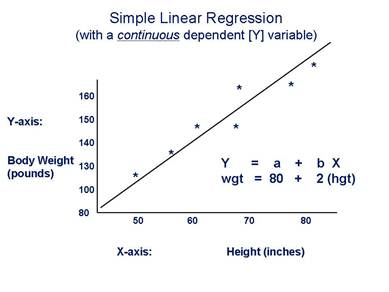
\includegraphics[center]{simpleLinearRegression}
	\caption[Confusion Matrix]
	{Simple Linear Regression}
	\label{fig:simpleLinearRegression}
\end{figure}

We can see from above the $Y$ in this example is weight (wgt) and $f(x)$ is $80 + 2*Height(hgt)$. This is a very basic example but demonstrates how this can be leveraged for more complex feature sets.

\subsection{Nearest Neighbours \& Distance Measures} \label{kNN}
When the \textit{k} nearest classifications are considered, 


\subsection{Decision Trees} \label{decTrees}
Decision Tree algorithms seek to split records into classes based on the inherent characteristics of the variables in the dataset and their relationship with the target variable(class).\\Prior to splitting the data, if we were to randomly pick a record from the dataset, the degree of uncertainty as to what class we would expect it to be would be relative to the distribution of the classes in the original dataset.


\subsection{Ensemble models \& Boosting} \label{boosting}
In 1907, statistician Sir Francis Galton attended a fair in which there was a competition to judge the weight of an Ox. Upon reviewing the 787 predictions made by the competing public, he observed that while there was a 





\subsection{Neural Networks} \label{neuralNets}
Neural Networks in broad terms are a class of model that attempt to learn patterns in data by simulating the activity in a human brain.


\subsection{Support Vector Machines} \label{SVM}
Support Vector Machines (SVM) were developed from Statistical Learning Theory 

\subsection{Sequential Association Rules, N-grams \& Markov Chains} \label{assosRules}
In their paper, introduce the concept of association rules for discovering statistically significant relationships between frequently occurring items in large datasets. The algorithm.
\subsection{Applications of Techniques in 2-Class Classification \& Path Prediction}\label{applic}
Compared using k-NN versus association rules as an approach to personalising recommendations on websites based on presenting users with pages that they are likely to visit next based on a history of page requests. The results showed that using association rules provided better coverage and precision than k-NN when they used a window of 4 previous page requests.

%----------------------------------------------------------------------------------------
%	SECTION 8
%----------------------------------------------------------------------------------------
\section{Class Imbalance Problem}
One of the biggest assumptions that needs to be understood when using classification algorithms is that most assume there is a balanced distribution of the target class \citep{japkowicz_class_2000}. Target class imbalance is described by  \citep{chawla_smote:_2002} where the number of number of records in each class are not relatively equal. In a balanced dataset ratio between the a binary target class would be close to 50/50. The issue with this imbalance arises where algorithms assume there is a balance between the classes, and they attempt to maximise the accuracy by predicting the most common class \citep{drummond_severe_2005}. The algorithms attempt to minimise the classification errors, but do not accounts for the incorrectly classifying cases \citep{seiffert_improving_2009}. While these classification overall might be very accurate they are not very useful in real world problems, this is because in the majority of cases the algorithm will focus on the majority class, because of how heavily it is weighted in the training dataset ignoring the minority class. This is major problem because in the majority of cases you will trying to predict the minority class, in this thesis customers going into default is the minority e.g. there are more customers that do not default at the end of the outcome window than customers that do defaulters.

As mentioned previously, very often in the real world problems imbalance exists in the dataset, thus there has been researched completed that have identified methods of mitigating against this risk. \citep{chawla_editorial:_2004} proposes solutions fine tuning the algorithm and manipulating the data. 

\subsection{Manipulating the data}

A method of manipulating the data is to resample to data with the aim of balancing the distribution of the target class. Solutions proposed,

\begin{itemize}
	\item Random undersampling the majority class
	\item Random oversampling the minority Class
	\item Synthetic of the minority Class 
\end{itemize}

A very common method used is to randomly oversample the minority class in your training set, one of the biggest issues with this is that you are increasing your chances of over-fitting the algorithm the training model as it been training on multiple copies of the same data which are not adding any new information. However over-fitting can be issue with this approach as the algorithm becomes biased and skewed on the training data, thus ends up performing poorly on the validation and test data \cite[see][]{hawkins_problem_2004}

Random undersampling of the minority class is where random samples of the training dataset that are part of the majority class are removed. This means number of minority classes remains unchanged but the majority class is reduced, thus the overall class balance becomes more even. The issue that arises from undersampling is that there is possibility that you removes the important information from the training dataset that is used for predicting that class. 

Synthetic sampling  is alternative method to randomly oversampling the minority class. New data items are added to the training set but unlike oversampling which adds duplicate records the records added are dummy or made up in a way to look similar and taking characteristics of the already existing records, thus they are not duplicates but synthetic. One method for creating synthetic data was proposed by \citep{chawla_smote:_2002} where data was generated by creating data items using K-NN where the item would sit between minority classes. 

\begin{figure}[H]
	\centering
	\begin{subfigure}[b]{0.32\textwidth}
		\captionsetup{font=scriptsize}
		\includegraphics[width=\textwidth]{SMOTE_Before}\caption{}
		\label{fig:SMOTE_Before}
	\end{subfigure}  ~\quad
	\begin{subfigure}[b]{0.32\textwidth}
		\captionsetup{font=scriptsize}
		\includegraphics[width=\textwidth]{SMOTE_After}
		\caption{}
		\label{fig:SMOTE_After}
	\end{subfigure}
\caption{Fig. \ref{fig:SMOTE_Before}: Example of the K-NN for $x_i$ using $k = 6$. \ref{fig:SMOTE_After}: Data created using SMOTE based on the euclidean distance.\\
	\cite[Source:][]{he_learning_2009}}
\label{fig:smoteExample}
\end{figure}

Above in Fig. \ref{fig:smoteExample} it is illustrated how synthetic data using the SMOTE methodology can be generated. For the purposes of this thesis this will not be discussed further.

\subsection{Fine tuning the algorithm}
There are ways to also cater for the target class imbalance of the dataset by fine tuning the algorithm. One method which is illustrated in Chapter \ref{Chapter4} of this thesis is to adjust the cut-off or threshold parameter value for the model, \cite{provost_machine_2000} warns that it would \textit{``critical mistake"}. In Section \ref{modelPerformMeasure} model performance measures, it is  worth noting that \cite{chawla_editorial:_2004} suggests using evaluation measures such as accuracy which rely on a specific threshold could lead to misleading results when the target class is imbalanced, they instead recommend using ROC and AUC to get a more accurate predictions, this similar to industry standards in terms of handling the imbalance.

This section has detailed some of the concern that imbalance can cause when building predictive models, we have outlined some the solutions and methods to mitigate this by manipulating the data and fine tuning the classification algorithm.

%----------------------------------------------------------------------------------------
%	SECTION 8
%----------------------------------------------------------------------------------------
\section{Model Validation Methods}
\url{"http://blog.dato.com/how-to-evaluate-ml-models-part-3-validation-and-offline-testing"}

\begin{itemize}
	\item Validation
	\item Offline Testing
	\item Online Testing
\end{itemize}

\subsubsection{Model Validation}
During model validation during testing/prototyping to fins tune classifier and analyse goodness of fit.

\subsubsection{Offline Testing}
Offline testing happens on a static past events, where the data is labelled dataset collected from past events. This is done to test deployed model is working correctly, it needs to be tested periodically.

\subsubsection{Offline testing vs. validation}
Model validation and offline testing both test the model’s performance, but they happen at different stages of the model’s life time. Validation is done to evaluate the goodness of fit of a learned model, which is a measurement of the quality of hyperparameters used during model training. (More on this in the next post on hyperparameter tuning.) Validation happens prior to real testing or deployment. Once the model is trained and deployed, we can continue to monitor its performance offline on a test dataset. This kind of offline batch testing does not require retraining the model. One can use a hold-out dataset for validation and another for offline testing, as long as the test set does not contain the validation set, this is fine. Cross validation, bootstrap and jackknife are resampling techniques that generate multiple random samples from the same dataset; they can be employed for validation or computing confidence intervals.

\subsubsection{Hold-out datasets}
Hold-out testing or validation is simple. Assuming that all data points are i.i.d. (independently and identically distributed), hold-out testing means one randomly holds out part of the data for testing. One trains the model on the larger portion of the data and evaluates test metrics on the smaller hold-out set. 

\subsubsection{Online Testing}
Online testing happens live in production, one example of this is known as A/B testing. Online testing is beyond the scope of this thesis so it will not be discussed further. 

\subsubsection{Cross validation}
Cross validation can be used when tuning the hyperparameters of the model. A lot of people seem to consider the two to be synonymous. But they are not. Cross validation is simply a way of generating training and validation sets for the process of hyperparameter tuning. Hold-out sets are also valid for hyperparameter tuning, and in fact they are computationally much cheaper.

There are many variants of cross validation. The most commonly known is k-fold cross validation. In this procedure, first one divides the training dataset into K folds. For a given a hyperparameter setting, one treats each of the k folds like a hold-out set, trains a model on the rest of the k-1 folds, and measures the quality of the model on the held-out fold. The overall performance is taken to be the average of the performance on all k folds. Repeat this procedure for all of the hyperparameter settings one wish to evaluate, then pick the hyperparameters that resulted in the highest k-fold average. Lastly, retrain the model on all k-folds (the entire training set).

Cross validation is useful when the training dataset is so small that one can’t afford to hold out part of the data just for validation purposes. With the size of modern datasets, this is rarely necessary. Hold-out validation is much faster and provides good estimates of model. This is what is currently implemented in GraphLab Create.

If one needs a variance on the validation score, then hold-out set may not suffice. Use cross validation, or bootstrap.

\subsubsection{some subsection}
When calculating a measure of model accuracy there are some considerations to be made to increase the likelihood of the model making accurate predictions on unseen data. If we build a model using the full historical dataset available and subsequently test the accuracy of the model against the same dataset then we are in danger of generating a model that is over-fitted to the training set and the accuracy observed from the subsequent test may be biased (i.e. optimistic of the accuracy of the model).

\subsubsection{Cross validation}

\subsubsection{Hold-out Datasets}



%----------------------------------------------------------------------------------------
%	SECTION 9
%----------------------------------------------------------------------------------------
\section{Model Performance Measures}\label{modelPerformMeasure}

This section details some of the metrics that can be used to assess the accuracy of a classifier. The result of the classification algorithm maps the modelled data into a category, in this thesis it a binary classifier that is output: 1 is output for identifying customers who will default (bad) or 0 is output for customers who will be not-default (good). The majority of classification algorithms will produce a ranked numeric value which can be converted to a binary representation by some threshold or cut-off decision driven from  the business objective that is trying to be optimised. This section will begin with a confusion matrix, details how this is leveraged to build other performance measures and details how charts and metrics can be leveraged together to decide on the performance measure to maximise the intended objective.

\url{http://www.saedsayad.com/model_evaluation_c.htm}

\subsubsection{Confusion Matrix}

The results that made by the classification algorithm can be represented by a contingency table known as a confusion matrix. In this thesis the classification algorithm will output a binary classification, so the confusion matrix will be made from a $2 \times 2$ matrix that has two classes, known as the \textit{positive} and \textit{negative} class. For this thesis, the positive class will be the customers that default and negative class will be the customers that do not default. It will illustrate what proportion of correct and incorrect predictions were made with respect to the target.The confusion matrix can be broken down into the following categories for this thesis:

\begin{itemize}
	\item \textit{true positive} (TP), cases that are predicted to default, and are {\color{green}{correctly}} classified as \textit{positive}
	\item \textit{false positive} (FP), cases that are predicted to default, and are {\color{red}{incorrectly}} classified as \textit{positive}, also known as \textit{Type I error}.
	\item \textit{false negative} (FN), cases that are predicted to not-default, and are {\color{red}{incorrectly}} classified as \textit{negative}, also known as \textit{Type II error}.
	\item  \textit{true negative} (TN), cases that are predicted to not default, and are {\color{green}{correctly}} classified \textit{negative}
	
\end{itemize}

Fig \ref{fig:ConfusionMatrix} illustrates how information from a confusion matrix can be presented and read.

\begin{figure}[H]
	\includegraphics[width=0.8\textwidth,center]{Confusion_Matrix}
	\caption[Confusion Matrix]
	{Confusion Matrix}
	\label{fig:ConfusionMatrix}
\end{figure}

Using the numbers outputted from the confusion matrix, model evaluation measures can calculated and evaluated for the required objective, measures such as \textit{accuracy} (Equation \ref{eq:Accuracy}) which measures proportion of the number of predictions that were correct, the \textit{misclassification rate} (Equation \ref{eq:Misclassification Rate}) what proportion of predictions were wrong, the \textit{sensitivity} (Equation \ref{eq:Sensitivity}), otherwise known as \textit{recall} or the \textit{true positive rate} (TPR), measures the proportion of the positive instances that are correctly identified i.e. proportion default cases that have been predicted correctly. \textit{Specificity} (Equation \ref{eq:Specificity}) measures the proportion of negative cases that are predicted correctly i.e. proportion of non-default cases that have been predicted correctly, \textit{precision} (Equation \ref{eq:precision}) measures when the classifier predict positive outcomes what proportion are correct, \textit{negative predictive value} (NPV) (Equation \ref{eq:npv}) measures the proportion of negative predictions that were correct i.e. if the classifier predicted the outcome would be non-default what proportion were correct. One measure that can be very useful when the where there is class imbalance is \textit{balance accuracy} (Equation \ref{eq:Balanaced Accuracy}), \citep{brodersen_balanced_2010} discusses how using this negates the impact of bias or skewness from the more frequent class

\begin{equation} \label{eq:Sensitivity}
\text{Sensitivity} = \text{Recall} = \frac{TP}{TP + FN}
\end{equation}

\begin{equation} \label{eq:Specificity}
\text{Specificity} = \frac{TN}{FP + TN}
\end{equation}

\begin{equation} \label{eq:precision}
\text{Precision} = \frac{TP}{TP + FP}
\end{equation}

\begin{equation} \label{eq:npv}
\text{Negative Predictive Value} = \frac{TN}{TN + FN}
\end{equation}

\begin{equation} \label{eq:Accuracy}
\text{Accuracy} = \frac{TP + TN}{TP + FP + FN + TN}
\end{equation}

\begin{equation} \label{eq:Balanaced Accuracy}
\text{Average Accuracy} = \text{Balanaced Accuracy} = \frac{Sensitivity + Specificity}{2}
\end{equation}

\begin{equation} \label{eq:Misclassification Rate}
\text{Misclassification Rate} =  \frac{FP + FN}{TP + FP + FN + TN} = 1 - \text{Accuracy}
\end{equation}

\begin{figure}[H]
	\includegraphics[width=0.8\textwidth,center]{Confusion_Matrix_Example}
	\caption[Confusion Matrix Example]
	{Confusion Matrix Example}
	\label{fig:ConfusionMatrixExample}
\end{figure}

Fig. \ref{fig:ConfusionMatrixExample} illustrates how the TP, FP, FN, TN can be used to create performance metrics for classification algorithm. As discussed already confusion matrix based performance measures are built on the threshold that is selected for converting the predicted numeric score into a binary outcome. Anecdotally you might believe that the cut-off or threshold of 0.50 is acceptable but this rule may not always especially if there is an imbalance between the positive and negative class in the dataset. The cut-off should should ideally be based on you business objective where you look to minimise, maximise and analyse the trade off as you alter the cut-off. 

The confusion matrix is not the only way to evaluate the performance of the classification algorithm and is not always advocated in the literature or by industry. In studies completed by \citep{lessmann_benchmarking_2008} choose not to select a classification cut-off arguing that studies comparing the same dataset and classifier could come to the different conclusions.

As mentioned in this section the confusion matrix measures the performance of classifier at a specific threshold, this can be leveraged to create graphical representations of the overall fitness of the model at any threshold. One such method that will be discussed in the next section is the \textit{receiver operating characteristic} (ROC). 


Confusion Matrix is used to evaluating a model where you have divided the output into distinct or discrete categories. A confusion matrix can be reconstructed for any point on the ROC curve. ROC is also is directly related to two other performance methods \textit{area under the curve} and \textit{gini} which will also be discussed.  

\subsubsection{ROC Chart, AUC and Gini Coefficient}
%\url{https://staesthetic.wordpress.com/2014/04/14/gini-roc-auc-and-accuracy/}
The ROC chart is used to evaluate and illustrate how well the evaluate the model fit, this can be a quick test to see if the model generalises well from the test data, to validation and test data. Fig. \ref{fig:ROC} illustrates on the \textit{x-axis} the false positive rate, and on the \textit{y-axis} the true positive rate is represented. As mentioned previously the points on the ROC chart are generated from confusion matrix built from many cut-off or threshold value between $\theta \in [0,1]$. Fig. \ref{fig:ROC} conceptually illustrates how the ROC chart is generated for varying thresholds. 

\begin{figure}[H]
	\includegraphics[width=0.8\textwidth,center]{ROC}
	\caption[ROC]
	{ROC Chart Example with thresholds 0.65 \& 0.50}
	\label{fig:ROC}
\end{figure}

Fig. \ref{fig:ROC} also illustrate how point (0,1) represents \textit{perfect classification}, that is the classifier correctly predicts all outcomes. 

The ROC chart is basically a combination of confusion matrices over many cut-off values of a classifier. As you can see above finite number of observations in the dataset dictates the number of thresholds that can be used to generate a ROC chart.

To compare ROC chart results of different classifiers the \textit{area under the ROC curve} (AUC) \citep{bradley_use_1997} \& \citep{hanley_meaning_1982}. In Fig. \ref{fig:ROC} the area under the blue ROC line represents the AUC, which is intuitively the area under the curve. In the case of perfect classification this value will be 1, for a random classifier the AUC would be 0.5. 

It is worth noting that AUC does not give total probability of the classifier, and also its usefulness when combined with the ROC to evaluate your classifier across training, validation and test datasets. For example if the ROC curve shifts significantly or is not similar from training to validation/test it suggests that there is possible over-fitting and the model does not generalise well. Also it is worth looking out for a drastic change in the AUC from training to validation/test another sign the classifier does not generalise well may not be useful for predictions. Because of this it is a very strong measure for classifier selection, ROC don't tend to cross over, therefore when comparing two classifiers the one which AUC is higher will be the better classifier independent of the threshold or cut-off.

It is illustrated in Fig. \ref{fig:matric_compare} how the performance measures for confusion matrices vary for different thresholds, but again to keep in mind that it there be just one measure for the AUC of the this ROC Chart.   

\begin{figure}[H]
	\centering
	\begin{subfigure}[b]{0.45\textwidth}
		\captionsetup{font=scriptsize}
		\includegraphics[width=\textwidth]{Confusion_Matrix_threshold_065}
		\caption{Threshold $=.65$}\label{fig:Threshold65}
	\end{subfigure} ~\quad
	\begin{subfigure}[b]{0.45\textwidth}
		\captionsetup{font=scriptsize}
		\includegraphics[width=\textwidth,height=2.025cm]{Confusion_Matrix_threshold_050}
		\caption{Threshold $=.50$}\label{fig:Threshold50}
	\end{subfigure}
	\caption{Confusion Matrix: Multiple Threshold Comparison}
	\label{fig:matric_compare}
\end{figure}

A metric that is commonly used for in \subjectname, industry credit scoring is the \textit{gini coefficient} this is discussed in \citep{hand_good_2005}, this is equates to twice the area in between the diagonal of a random classifier and the ROC curve. The equation for this can be seen below in Equation \ref{eq:gini}

\begin{equation} \label{eq:gini}
\text{Gini} = 2*\text{AUC} - 1
\end{equation}

Just like using a threshold there are limitations to using the AUC and Gini to measure classifier performance, although extremely useful for analysing the performance of wide range of thresholds but not as useful when trying to maximise the performance over a narrow range of thresholds. It cannot tell us the optimal threshold for classifier for  other statistical needs.

One statistic that is commonly used in credit scoring in \subjectname\, industry and in the literature is the \textit{kolmogorov-smirnov} (KS) statistic, this will be discussed in the next subsection.
	

\subsubsection{K-S Chart}\label{subsub:ks}
%\url{http://www.saedsayad.com/model_evaluation_c.htm}
The KS chart and more specifically the KS statistic is one value between 0 and 1. It can be used by measuring the performance of the classifier, by measuring the maximum distance between the cumulative positive and negative distributions of the predicted positive and negative class \citep{seliya_study_2009}. In other words K-S is a measure that illustrates the maximum seperation between the positive and negative distributions, this can illustrated more clearly in Fig. \ref{fig:ks}.

Fig. \ref{fig:ks} how the KS statistic and chart is generated, probabilities from the classifier are ordered, grouped and aggregated, but importantly they are separated by the positive and negative class, creating a distribution for each. These two distributions are then plotted separately, you can see in Fig. \ref{fig:ks} that the KS statistic is 47.4\%. This is calculated by taking maximum difference between the two distributions at each group. At group 400-500, if you were to classify all the score are positive below or in this group you would be identifying 81.7\% of the positive instance and only 34.3\% of the negative class, if this was a balanced dataset this could be a very valuable result and measure. 

\begin{figure}[H]
	\includegraphics[width=0.8\textwidth,center]{ks}
	\caption[Kolmogorov-Smirnov chart ]
	{Kolmogorov-Smirnov Table \& Chart }
	\label{fig:ks}
\end{figure}

There are extreme cases of the KS statistic that are worth noting, on is where the KS statistic is equal to 100, this means the scores for each distribution (positive/negative) are but into two separate groups, where one group would just have positive cases and the other just negative case. Alternatively if the model is not very useful and cannot tell the positives from the negatives, it will be like the model is selecting cases randomly and will return a KS statistic of 0.

We will see Chapter \ref{Chapter4} how this statistic can be utilised and leveraged to create a useful threshold value. 

\subsubsection{Gain \& Lift}
The \textit{gain} \& \textit{lift} measure the performance of the classifier. One example where these measure as charts are extremely useful is when communicating in industry with management, they are easy to explain and intuitive where the business can derive and understand value immediately. Fig. \ref{fig:GainLiftWorkflowCharts} below illustrates how the gain and lift charts are generated. 

\begin{figure}[H]
	\centering
	\begin{subfigure}[b]{0.90\textwidth}
		\captionsetup{font=scriptsize}
		\includegraphics[width=\textwidth,height=4cm]{gains_ratio_process}\caption{Process}\label{fig:gains_ratio_process}
	\end{subfigure} 
	\medskip
	\newline
	\begin{subfigure}[b]{0.45\textwidth}
		\captionsetup{font=scriptsize}
		\includegraphics[width=\textwidth]{gains}
		\caption{Gain Chart}\label{fig:gains}
	\end{subfigure} ~\quad
	\begin{subfigure}[b]{0.45\textwidth}
		\captionsetup{font=scriptsize}
		\includegraphics[width=\textwidth]{lift}
		\caption{Lift Chart}\label{fig:lift}
	\end{subfigure}
	\caption{Gain \& Lift Work-flow \& Charts}
	\label{fig:GainLiftWorkflowCharts}
\end{figure}

The charts above illustrate how much likely it is we receive positive responses using the classifier compared to use a random model. The population in the dataset are broken into deciles, which can be seen in \ref{fig:gains} \& \ref{fig:lift}. An example of how they can be used is if we were to evaluate the first 10\% of the population identified by the classifier it would outperform a random selection of customers that would turn out to positive by 3.6.

Essentially these charts are visual aids which can be leveraged for evaluating the performance of the classifier. 

%----------------------------------------------------------------------------------------
%	SECTION 5
%----------------------------------------------------------------------------------------
\section{Conclusion}\label{sotaConc}
This chapter has summarised the relevant literature available for two-class classification and web data analysis, with discussion of predicting future behaviour based on sequential click patterns. Various models have been discussed including K-Nearest Neighbours, Association Rules, Decision Trees, SVM, Neural Networks, Regression Models and ensemble models

%----------------------------------------------------------------------------------------
%	SECTION 6
%----------------------------------------------------------------------------------------
